\chapter{Pruebas y resultados\label{sec:resultados}}

\section{Introducción}
Tras el diseño y la implementación del sistema \textit{big data}, se procederá con la realización de conjuntos de baterías de pruebas en los diferentes entornos con el fin de estudiar su escalabilidad, comparar su rendimiento y detectar limitaciones del sistema. 

Estas pruebas se realizarán teniendo en cuenta dos factores, por un lado, el tamaño del fichero a procesar, es decir, partiendo del archivo completo se generarán otros ficheros parciales de menor tamaño con el objetivo de detectar el umbral donde el uso de un sistema distribuido pasa a ser efectivo. Por otro lado, utilizaremos distintas configuraciones del sistema para comparar su eficiencia, variando el número de procesadores (\gls{CPU}) y la cantidad de \gls{RAM}.

Estas pruebas serán complementarias, es decir, se realizarán para todos los sistemas de forma simultánea. Con respecto a las configuraciones del sistema \textit{big data} diseñadas, para realizar las pruebas, utilizaremos dos de ellas. Primero estableceremos el sistema en modo pseudo-distribuido y, posteriormente, en modo multinodo. Estas, se realizaran tanto en el clúster doméstico como en el universitario.

\section{Entorno de prueba}
En este apartado se detallarán las características de las máquinas utilizadas para cada configuración del sistema \textit{big data}.

\subsection{Configuración pseudo-distribuida}
En este modo solo existe una máquina que ejerce como maestro y esclavo. Esta configuración se ha establecido tanto para el clúster doméstico como el universitario.

\subsubsection{Clúster doméstico \label{pseudodomestico}}
Cuyas especificaciones están reflejadas en la tabla \ref{maestroDomestico}.

\begin{table}[htp!]
	\centering
	\caption{Especificaciones maestro en el clúster doméstico}
	\label{maestroDomestico}
	\begin{tabular}{|l|l|}
		\hline
		\multicolumn{2}{|c|}{\textbf{GENERAL}}                                 \\ \hline
		\textbf{Nombre:}            & PORTATILINUX                             \\ \hline
		\textbf{Sistema Operativo:} & Linux                                    \\ \hline
		\textbf{Versión:}           & Ubuntu 16.10 (64 bits)                   \\ \hline
		\textbf{Usuario:}           & adrigrillo                               \\ \hline
		\multicolumn{2}{|c|}{\textbf{SISTEMA}}                                 \\ \hline
		\textbf{Procesador:}        & Intel(R) Core(TM) i7-3537U CPU @ 2.00GHz \\ \hline
		\textbf{Cores:}             & 2                                        \\ \hline
		\textbf{Threads por core:}  & 2                                        \\ \hline
		\textbf{RAM:}               & 8192                                     \\ \hline
		\multicolumn{2}{|c|}{\textbf{ALMACENAMIENTO}}                          \\ \hline
		\textbf{Dispositivo:}       & Kingston SUV400S37480G                   \\ \hline
		\textbf{Tamaño:}            & 500 GB                                   \\ \hline
		\multicolumn{2}{|c|}{\textbf{RED}}                                     \\ \hline
		\textbf{Dispositivo:}       & Realtek PCIe GBE Family Controller       \\ \hline
		\textbf{Nombre:}            & Master                                   \\ \hline
	\end{tabular}
\end{table}

\subsubsection{Clúster universitario}
Cuyas especificaciones están reflejadas en la tabla \ref{equipoUniversitario}.
\begin{table}[htp!]
	\centering
	\caption{Especificaciones de los equipos en el clúster universitario.}
	\label{equipoUniversitario}
	\begin{tabular}{|l|l|}
		\hline
		\multicolumn{2}{|c|}{\textbf{GENERAL}}                                      \\ \hline
		\textbf{Nombre:}            & it0XX/lm0XX                                   \\ \hline
		\textbf{Sistema Operativo:} & Linux                                         \\ \hline
		\textbf{Versión:}           & Debian GNU/Linux 8.1                          \\ \hline
		\textbf{Usuario:}           & 316457                                        \\ \hline
		\multicolumn{2}{|c|}{\textbf{SISTEMA}}                                      \\ \hline
		\textbf{Procesador:}        & Intel(R) Core(TM) i3-3240 CPU @ 3.40GHz       \\ \hline
		\textbf{Cores:}             & 2                                             \\ \hline
		\textbf{Threads por core:}  & 2                                             \\ \hline
		\textbf{RAM:}               & 8192                                          \\ \hline
		\multicolumn{2}{|c|}{\textbf{ALMACENAMIENTO}}                               \\ \hline
		\textbf{Dispositivo:}       & ATA WDC WD5000AAKX-0 \\ \hline
		\textbf{Tamaño:}            & 30 GB                                         \\ \hline
		\multicolumn{2}{|c|}{\textbf{RED}}                                          \\ \hline
		\textbf{Dispositivo:}       & Qualcomm Atheros AR8161 Gigabit Ethernet      \\ \hline
		\textbf{Nombre:}            & it0XX/lm0XX                                   \\ \hline
	\end{tabular}
\end{table}

\subsection{Configuración multinodo}
En esta configuración habrá un maestro que será el que controle a los demás ordenadores del sistema, distribuyendo las tareas entre los esclavos, controlando los procesos y recogiendo los resultados obtenidos por estos. 

Aunque la función principal del maestro sea controlar la ejecución y distribuir las tareas, por su parte, el también dedicará recursos para el procesamiento de la información, de forma muy similar a la configuración pseudo-distribuida.

\subsubsection{Clúster doméstico \label{especifDom}}
El clúster doméstico estará formado por tres ordenadores, cada uno con sus propias especificaciones. En esta configuración contaremos con tres máquinas, un maestro y dos esclavos, que, en teoría, es tres veces más potente que la configuración pseudo-distribuida doméstica \ref{pseudodomestico} al contar con tres veces más \gls{CPU} y cantidad de \gls{RAM}.

Esta se compondrá por:

\begin{itemize}
	\item \textbf{Maestro:} será el mismo usado en la configuración pseudo-distribuida, con las características comentadas en la tabla \ref{maestroDomestico}.
	
	\item \textbf{Esclavo 1:} Cuyas características se encuentran en la tabla \ref{esclavo1}.

	\item \textbf{Esclavo 2:} Cuyas características se encuentran en la tabla \ref{esclavo2}.
\end{itemize}
\begin{table}[htp!]
	\centering
	\caption{Especificaciones esclavo 1 en el clúster doméstico}
	\label{esclavo1}
	\begin{tabular}{|l|l|}
		\hline
		\multicolumn{2}{|c|}{\textbf{GENERAL}}                                                                \\ \hline
		\textbf{Nombre:}            & SobreMesa                                                               \\ \hline
		\textbf{Sistema Operativo:} & Linux                                                                   \\ \hline
		\textbf{Versión:}           & Ubuntu 16.10 (64 bits)                                                  \\ \hline
		\textbf{Usuario:}           & adrigrillo                                                              \\ \hline
		\multicolumn{2}{|c|}{\textbf{SISTEMA}}                                                                \\ \hline
		\textbf{Procesador:}        & Intel(R) Core(TM)2 Quad CPU    Q6600  @ 2.40GHz                         \\ \hline
		\textbf{Cores:}             & 4                                                                       \\ \hline
		\textbf{Threads por core:}  & 1                                                                       \\ \hline
		\textbf{RAM:}               & 4096                                                                    \\ \hline
		\multicolumn{2}{|c|}{\textbf{ALMACENAMIENTO}}                                                         \\ \hline
		\textbf{Dispositivo:}       & ATI SB600 Non-Raid-5 SATA                                               \\ \hline
		\textbf{Tamaño:}            & 500 GB                                                                  \\ \hline
		\multicolumn{2}{|c|}{\textbf{RED}}                                                                    \\ \hline
		\textbf{Dispositivo:}       & Marvell Technology Group Ltd. 88E8056 PCI-E \\ \hline
		\textbf{Nombre:}            & Esclavo1                                                                \\ \hline
	\end{tabular}
\end{table}

\begin{table}[htp!]
	\centering
	\caption{Especificaciones esclavo 2 en el clúster doméstico}
	\label{esclavo2}
	\begin{tabular}{|l|l|}
		\hline
		\multicolumn{2}{|c|}{\textbf{GENERAL}}                                 \\ \hline
		\textbf{Nombre:}            & Linux2                                   \\ \hline
		\textbf{Sistema Operativo:} & Linux                                    \\ \hline
		\textbf{Versión:}           & Ubuntu 16.10 (64 bits)                   \\ \hline
		\textbf{Usuario:}           & adrigrillo                               \\ \hline
		\multicolumn{2}{|c|}{\textbf{SISTEMA}}                                 \\ \hline
		\textbf{Procesador:}        & Intel(R) Core(TM) i5-6200U CPU @ 2.50GHz \\ \hline
		\textbf{Cores:}             & 2                                        \\ \hline
		\textbf{Threads por core:}  & 2                                        \\ \hline
		\textbf{RAM:}               & 12288                                    \\ \hline
		\multicolumn{2}{|c|}{\textbf{ALMACENAMIENTO}}                          \\ \hline
		\textbf{Dispositivo:}       & HDD.9.5mm.1TB.5K4.SATA2.4K               \\ \hline
		\textbf{Tamaño:}            & 1 TB                                     \\ \hline
		\multicolumn{2}{|c|}{\textbf{RED}}                                     \\ \hline
		\textbf{Dispositivo:}       & Realtek PCIe GBE Family Controller       \\ \hline
		\textbf{Nombre:}            & Esclavo2                                 \\ \hline
	\end{tabular}
\end{table}

\subsubsection{Clúster universitario}
\label{clusterUni}
En esta configuración utilizaremos los laboratorios de telemática para implementar el sistema \textit{big data}. Esto es positivo ya que todos los ordenadores utilizados tienen las mismas características (tabla \ref{equipoUniversitario}) por lo que el clúster será ideal debido a la homogeneidad de los equipos.

Para las pruebas utilizaremos diferentes configuraciones variando el número de dispositivos conectados al sistema \textit{big data}. Para establecer el número de los mismos en cada configuración utilizaremos una evolución lineal, utilizando finalmente las siguientes:

\begin{itemize}
	\item Clúster de 2 ordenadores, 8 \gls{CPU}s y 16 GB de \gls{RAM}.
	\item Clúster de 4 ordenadores, 16 \gls{CPU}s y 32 GB de \gls{RAM}.
	\item Clúster de 8 ordenadores, 32 \gls{CPU}s y 64 GB de \gls{RAM}.
	\item Clúster de 16 ordenadores, 64 \gls{CPU}s y 128 GB de \gls{RAM}.
\end{itemize}

Con estas configuraciones, vemos como los recursos se doblan en cada prueba por lo que, idealmente, veríamos como los tiempos se reducen a la mitad con cada configuración.

\section{Fichero de datos \label{compFichDatos}}
La eficiencia del sistema y, por tanto, su conveniencia de uso, es decir, su rentabilidad, también dependen del formato y tamaño de los datos a procesar y la complejidad computacional del proceso a realizar. 

Por ello, además de modificar las diferentes configuraciones de equipos, también vamos a realizar un estudio sobre el tipo de fichero donde se almacenarán los datos y el comportamiento del sistema con diferentes tamaños del archivo y tareas que debe realizar el sistema, que son el procesamiento de datos y las consultas.

En cuanto al formato utilizado para los ficheros de datos, vamos a comparar entre tener los datos almacenados en un fichero \textit{\gls{CSV}} o utilizar \textit{Apache Parquet}, cuyas ventajas e inconvenientes se han comentado anteriormente en el apartado \ref{parquetBeneficios}. En nuestro caso, para las tareas que realizará nuestro sistema, que serán consultas sobre los datos existentes sin modificar los datos, lo que más nos interesa es la velocidad de lectura. Por ello, procederemos a realizar pruebas de lectura para comparar la velocidad entre los dos formatos.


Con respecto al tamaño de los datos, partiendo del \gls{CSV} original, creamos diferentes archivos de menor tamaño para comprobar a partir de que punto montar una arquitectura \textit{big data} pasa a ser eficiente. La creación de estos ficheros no se realiza con respecto al tamaño del fichero en megas, si no, teniendo en cuenta el número de registros en el fichero. 

En las siguientes tablas se muestra el tamaño en disco y el número de registros de los ficheros creados. En concreto, la tabla \ref{ficherosCSV} son los archivos \textit{\gls{CSV}} utilizados y la tabla \ref{ficherosParquet} son los archivos en formato \textit{parquet}.

\begin{table}[htp!]
	\centering
	\caption{Ficheros \gls{CSV} empleados.}
	\label{ficherosCSV}
	\begin{tabular}{|l|l|l|}
		\hline
		\multicolumn{3}{|c|}{\textbf{CSV}}                          \\ \hline
		\textbf{Nombre} & \textbf{Registros} & \textbf{Tamaño (GB)} \\ \hline
		mil.csv         & 173185             & 0,032519531          \\ \hline
		quinientos.csv  & 346370             & 0,065039063          \\ \hline
		cinquenta.csv   & 3463702            & 0,649707031          \\ \hline
		1decimo.csv     & 17318509           & 3,3                  \\ \hline
		2decimo.csv     & 34637018           & 6,7                  \\ \hline
		3decimo.csv     & 51955527           & 10                   \\ \hline
		4decimo.csv     & 69274036           & 13,3                 \\ \hline
		half.csv        & 86592546           & 16,6                 \\ \hline
		6decimo.csv     & 103911055          & 20                   \\ \hline
		7decimo.csv     & 121229563          & 23,3                 \\ \hline
		8decimo.csv     & 138548072          & 26,6                 \\ \hline
		9decimo.csv     & 155866581          & 30                   \\ \hline
		full.csv        & 173185091          & 33,3                 \\ \hline
	\end{tabular}
\end{table}

\begin{table}[htp!]
	\centering
	\caption{Ficheros .parquet empleados.}
	\label{ficherosParquet}
	\begin{tabular}{|l|l|l|}
		\hline
		\multicolumn{3}{|c|}{\textbf{Apache Parquet}}             \\ \hline
		\textbf{Nombre}    & \textbf{Registros} & \textbf{Tamaño} \\ \hline
		mil.parquet        & 166570             & 0,0078125       \\ \hline
		quinientos.parquet & 333971             & 0,012304688     \\ \hline
		cinquenta.parquet  & 3341159            & 0,089160156     \\ \hline
		1decimo.parquet    & 16716605           & 0,44140625      \\ \hline
		2decimo.parquet    & 33428358           & 0,883789063     \\ \hline
		3decimo.parquet    & 50192489           & 1,32            \\ \hline
		4decimo.parquet    & 66932537           & 1,76            \\ \hline
		half.parquet       & 83216713           & 2,2             \\ \hline
		6decimo.parquet    & 100048869          & 2,65            \\ \hline
		7decimo.parquet    & 116946068          & 3,11            \\ \hline
		8decimo.parquet    & 133836035          & 3,56            \\ \hline
		9decimo.parquet    & 150630563          & 4,01            \\ \hline
		full.parquet       & 167361464          & 4,46            \\ \hline
	\end{tabular}
\end{table}

\section{Resultados de las consultas}
Aunque el objetivo principal de este trabajo es analizar y comparar el comportamiento de las diferentes configuraciones de la arquitectura \textit{big data} diseñada e implementada, este toma como inspiración el desafío planteado en la convocatoria del \gls{DEBS} \cite{grandChallenge} y, por ello, realiza las consultas planteadas en el mismo.

Las consultas sobre los datos planteadas en el concurso y realizadas para este trabajo ya han sido comentadas en detalle anteriormente en el apartado \ref{impConsultas}. En esencia, estas son obtener las rutas más frecuentes y las zonas donde un taxista puede lograr más beneficio, ambas, dentro de una franja de tiempo.

En el concurso, los resultados se pedían en fichero de texto con un formato establecido, donde se devolvía franja horaria donde se realiza la consulta, el resultado de la consulta, con las diez rutas más frecuentes o las diez zonas que más beneficios aportarían, y el tiempo llevado por la consulta para realizarse. En este caso, para el trabajo, también hemos seguido estas indicaciones y los resultados se devuelven en archivos de texto plano.

Debido a la falta de resultados comprobados, no ha sido posible cotejar los datos obtenidos en las consultas implementadas y ejecutadas. Por tanto, en lo que nos fijaremos es que las pruebas den los mismos resultados independientemente de la configuración del sistema, es decir, que la ejecución en paralelo no altere los resultados.

Para la consulta de las rutas más frecuentes para el 1 de enero a las 9:45 de la mañana, obtenemos los siguientes resultados:

\begin{verbatim}
# 1 ordenador
2013-01-01 09:15:00, 2013-01-01 09:45:00, 0: (156, 160) (155, 162), 
1: (157, 163) (155, 162), 2: (157, 160) (155, 162), 
3: (158, 161) (155, 162), 4: (162, 156) (155, 162), 
5: (155, 161) (157, 160), 6: (155, 162) (157, 162), 
7: (155, 163) (153, 161), 8: (158, 162) (155, 162), 
9: (162, 155) (155, 162), 84,8223688602

# 2 ordenadores
2013-01-01 09:15:00, 2013-01-01 09:45:00, 0: (156, 160) (155, 162), 
1: (157, 163) (155, 162), 2: (157, 160) (155, 162), 
3: (158, 161) (155, 162), 4: (155, 161) (157, 160), 
5: (155, 162) (157, 162), 6: (162, 156) (155, 162), 
7: (155, 163) (153, 161), 8: (156, 161) (152, 171), 
9: (162, 155) (155, 162), 22,42932355300036

# 4 ordenadores
2013-01-01 09:15:00, 2013-01-01 09:45:00, 0: (156, 160) (155, 162), 
1: (157, 163) (155, 162), 2: (157, 160) (155, 162), 
3: (158, 161) (155, 162), 4: (162, 156) (155, 162), 
5: (155, 161) (157, 160), 6: (155, 162) (157, 162), 
7: (155, 163) (153, 161), 8: (158, 162) (155, 162), 
9: (162, 155) (155, 162), 19,517775600999812

# 8 ordenadores
2013-01-01 09:15:00, 2013-01-01 09:45:00, 0: (156, 160) (155, 162), 
1: (157, 163) (155, 162), 2: (157, 160) (155, 162), 
3: (158, 161) (155, 162), 4: (155, 161) (157, 160), 
5: (155, 162) (157, 162), 6: (162, 156) (155, 162), 
7: (155, 163) (153, 161), 8: (155, 160) (154, 162), 
9: (156, 161) (152, 171), 16,43703933299912

# 16 ordenadores
2013-01-01 09:15:00, 2013-01-01 09:45:00, 0: (156, 160) (155, 162), 
1: (158, 161) (155, 162), 2: (157, 160) (155, 162), 
3: (157, 163) (155, 162), 4: (155, 162) (157, 162), 
5: (155, 161) (157, 160), 6: (162, 156) (155, 162), 
7: (155, 163) (153, 161), 8: (155, 160) (154, 162), 
9: (162, 155) (155, 162), 14,15684618800151
\end{verbatim}

Para el caso de las zonas que más beneficios reportan el 1 de enero a las 9:45 de la mañana obtenemos los siguientes resultados:

\begin{verbatim}
# 1 ordenador
2013-01-01 09:15:00, 2013-01-01 09:45:00, 0: (166, 158) 1: (179, 154) 
2: (184, 152) 3: (157, 167) 4: (137, 166) 5: (152, 162) 6: (170, 164) 
7: (177, 160) 8: (167, 161) 9: (144, 162) 196,630329132

# 2 ordenadores
2013-01-01 09:15:00, 2013-01-01 09:45:00, 0: (166, 158) 1: (179, 154) 
2: (184, 152) 3: (157, 167) 4: (137, 166) 5: (152, 162) 6: (170, 164) 
7: (177, 160) 8: (167, 161) 9: (144, 162) 54,310519398

# 4 ordenadores
2013-01-01 09:15:00, 2013-01-01 09:45:00, 0: (166, 158) 1: (179, 154) 
2: (184, 152) 3: (157, 167) 4: (137, 166) 5: (152, 162) 6: (170, 164) 
7: (177, 160) 8: (167, 161) 9: (144, 162) 51,68224776399984

# 8 ordenadores
2013-01-01 09:15:00, 2013-01-01 09:45:00, 0: (166, 158) 1: (179, 154) 
2: (184, 152) 3: (157, 167) 4: (137, 166) 5: (152, 162) 6: (170, 164) 
7: (177, 160) 8: (167, 161) 9: (144, 162) 37,54356300600193

# 16 ordenadores
2013-01-01 09:15:00, 2013-01-01 09:45:00, 0: (166, 158) 1: (179, 154) 
2: (184, 152) 3: (157, 167) 4: (137, 166) 5: (152, 162) 6: (170, 164) 
7: (177, 160) 8: (167, 161) 9: (144, 162) 34,71620901699862
\end{verbatim}

Una vez obtenidos los resultados, vemos como en el caso de las rutas más frecuentes, los resultados son diferentes dependiendo de la ejecución y, sin embargo, en el caso de las zonas que más beneficios pueden reportar los resultados son siempre iguales.

Esto podría hacer pensar que la primera consulta está mal elaborada, sin embargo, tras hacer la comprobación de los resultados descubrimos que no es así. La explicación de esto es que existen ciertas rutas que a dicha hora se realizan el mismo número de veces, por tanto, dependiendo del tiempo en el que el maestro reciba los resultados estos se situarán antes o después en la lista final.

De hecho, si nos fijamos en el proceso que realiza la consulta (explicado en el punto \ref{freqSinExplicacion}) esta no es más que un filtrado para tomar los datos de la franja horaria y un \textit{count} de los datos. Por ello, podemos encontrar que los primeros dos resultados son siempre los mismo, aunque, posteriormente, las rutas que se han realizado el mismo número de veces dependerán del reparto de los datos entre los esclavos.

Con respecto a la segunda consulta, que depende de más datos y cálculos que la primera (explicado en el punto \ref{profSinExplicacion}) es más complicado que los resultados entre dos zonas sean los mismos, por ello, siempre tienen el mismo orden en el fichero de salida, independientemente de la configuración del sistema.

Por ello, y, a falta de una forma de comprobar si los datos obtenidos son correctos, damos por finalizado el análisis de los resultados obtenidos.

\section{Rendimiento de los formatos del fichero de datos \label{resCompFich}}
Como se ha comentado en la implementación, en el apartado \ref{anaProcData}, aunque el fichero de datos original se ofrecía como un \textit{\gls{CSV}} de 33 GB, que era totalmente compatible con las tecnologías usadas, uno de los objetivos del trabajo era obtener la mayor eficiencia del sistema, por ello se decidió utilizar \textit{Apache Parquet} como formato para almacenar los datos en el disco, ante la promesa de mayor velocidad de lectura y menor uso de espacio en el disco.

Para comparar ambos formatos, se han realizado pruebas de lectura sobre los archivos utilizados en el sistema (Tablas \ref{ficherosCSV} y \ref{ficherosParquet}). Estas consisten en un \textit{count} de todos los registros presentes en los ficheros, tomando los tiempos que ha tomado hacer cada lectura individual y el total de todas.

Los resultados obtenidos en las pruebas se pueden apreciar en la tabla \ref{velocidadCSV} para los ficheros \gls{CSV} y en la tabla \ref{velocidadParquet} para los \textit{Parquet}.

\begin{table}[htp!]
	\centering
	\caption{Pruebas de lectura para formato \gls{CSV}}
	\label{velocidadCSV}
	\begin{tabular}{|l|l|l|l|l|}
		\hline
		\multicolumn{5}{|c|}{\textbf{CSV}}                                                                               \\ \hline
		\textbf{Nombre} & \textbf{Registros} & \textbf{Tamaño (GB)} & \textbf{Tiempo (seg)} & \textbf{Registros/seg} \\ \hline
		mil.csv         & 173185             & 0,032519531     & 0,99720043                 & 173671                     \\ \hline
		quinientos.csv  & 346370             & 0,065039063     & 1,959946904                & 176724                     \\ \hline
		cinquenta.csv   & 3463702            & 0,649707031     & 15,24788392                & 227159                     \\ \hline
		1decimo.csv     & 17318509           & 3,3             & 494,5507809                & 35018                      \\ \hline
		2decimo.csv     & 34637018           & 6,7             & 389,0821234                & 89022                      \\ \hline
		3decimo.csv     & 51955527           & 10              & 291,1400167                & 178455                     \\ \hline
		4decimo.csv     & 69274036           & 13,3            & 182,5482055                & 379483                     \\ \hline
		half.csv        & 86592546           & 16,6            & 86,86696803                & 996840                     \\ \hline
		6decimo.csv     & 103911055          & 20              & 585,2277942                & 177556                     \\ \hline
		7decimo.csv     & 121229563          & 23,3            & 703,9244393                & 172219                     \\ \hline
		8decimo.csv     & 138548072          & 26,6            & 827,5500103                & 167419                     \\ \hline
		9decimo.csv     & 155866581          & 30              & 952,5683697                & 163627                     \\ \hline
		full.csv        & 173185091          & 33,3            & 978,0770412                & 177066                     \\ \hline
		&                    &                      & \textbf{Tiempo total (seg)} & \textbf{Media reg/seg}     \\ \hline
		&                    &                 & 5509,740781                & 239558,3846                \\ \hline
	\end{tabular}
\end{table}

\begin{table}[htp!]
	\centering
	\caption{Pruebas de lectura para formato \textit{Parquet}}
	\label{velocidadParquet}
	\begin{tabular}{|l|l|l|l|l|}
		\hline
		\multicolumn{5}{|c|}{\textbf{PARQUET + SNAPPY}}                                                                          \\ \hline
		\textbf{Nombre}    & \textbf{Registros} & \textbf{Tamaño (GB)} & \textbf{Tiempo (seg)} & \textbf{Registros/seg} \\ \hline
		mil.parquet        & 166570             & 0,0078125            & 0,088930148                 & 1873043                    \\ \hline
		quinientos.parquet & 333971             & 0,012304688          & 0,10375922                  & 3218711                    \\ \hline
		cinquenta.parquet  & 3341159            & 0,089160156          & 0,13233389                  & 25247946                   \\ \hline
		1decimo.parquet    & 16716605           & 0,44140625           & 0,533758281                 & 31318680                   \\ \hline
		2decimo.parquet    & 33428358           & 0,883789063          & 1,172321222                 & 28514674                   \\ \hline
		3decimo.parquet    & 50192489           & 1,32                 & 1,802668324                 & 27843440                   \\ \hline
		4decimo.parquet    & 66932537           & 1,76                 & 2,563482635                 & 26110002                   \\ \hline
		half.parquet       & 83216713           & 2,2                  & 3,21071474                  & 25918438                   \\ \hline
		6decimo.parquet    & 100048869          & 2,65                 & 3,437491023                 & 29105201                   \\ \hline
		7decimo.parquet    & 116946068          & 3,11                 & 6,598058132                 & 17724316                   \\ \hline
		8decimo.parquet    & 133836035          & 3,56                 & 10,72142728                 & 12483042                   \\ \hline
		9decimo.parquet    & 150630563          & 4,01                 & 8,413226073                 & 17904019                   \\ \hline
		full.parquet       & 167361464          & 4,46                 & 19,46584598                 & 8597697                    \\ \hline
		                   &                    &                      & \textbf{Tiempo total (seg)} & \textbf{Media reg/seg}     \\ \hline
						   &                    &                      & 58,24401784                 & 19681477,62                \\ \hline
	\end{tabular}
\end{table}

A la vista de los resultados obtenidos, destaca la gran diferencia que existe entre los dos formatos tanto en espacio ocupado en disco, donde los archivos \textit{.parquet} son un 85\% más ligeros, como en velocidad de lectura, donde es un 8215\% más rápido.

Si bien los resultados en cuanto a espacio son muy buenos, son más esperados debido al uso del sistema de compresión \textit{snappy} durante el guardado y uso de los archivos, que es soportado de forma nativa por parte del \Gls{framework}. Como es lógico, al comprimir los archivos, estos ocuparán menos en el disco. En la gráfica \ref{gra:espacioFichero} se puede apreciar más claramente esta diferencia.

Sin embargo, la gran diferencia entre la velocidad de lectura de los formatos no se esperaba tan alta, aunque si tienen sentido. Por un lado, debido a que se trata de un \textit{count} de los registros y el almacenamiento es a base de columnas, no es necesario leer toda la línea de datos del registro, si no solo uno de sus atributos para contarlo como válido, reduciendo la cantidad de datos a leer del disco.

Por otro lado, el uso de mecanismos de compresión hace que el acceso a datos necesarios del disco duro, que es una operación lenta, sea mucho menor, haciendo que con muchos menos accesos se realice la lectura del fichero completo. Si bien es cierto que esto se produce a costa de un mayor esfuerzo de la \gls{CPU}.

Esto confirma que el uso de un sistema de almacenamiento columnar junto con un mecanismo eficiente de compresión es efectivo para tareas de lectura de datos. Por ello, debido al resultado de las mismas y a la naturaleza de los procesos que se realizan en este trabajo, que son mayoritariamente de lectura y de operaciones con columnas, se decidió utilizar este tipo de ficheros.

\begin{figure}[htp!]
	\centering
	\caption{Evolución tamaño fichero con respecto al número de registros}
	\label{gra:espacioFichero}
	\vspace{5pt}
	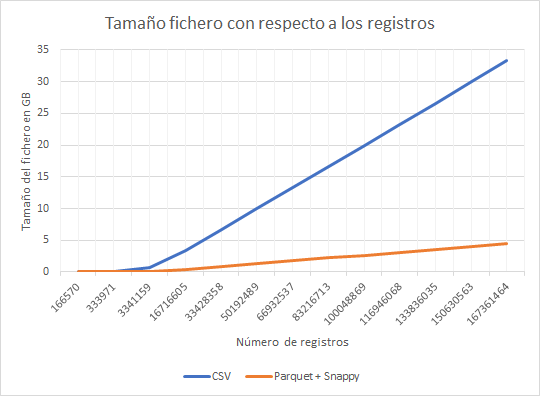
\includegraphics[scale=1]{graficas/espacioFichero}
\end{figure}

\section{Eficiencia de la infraestructura}
Una vez comentados los resultados obtenidos y las pruebas realizadas sobre los ficheros de datos, vamos a proceder a analizar el rendimiento del sistema \textit{big data} con las diferentes configuraciones implementadas. 

Primero comentaremos los resultados obtenidos en el clúster doméstico y, posteriormente, pasaremos a analizar los resultados en el clúster universitario, que son más representativos al tener mayor similitud con un sistema más realista.

En ambos realizaremos todas las pruebas, primero el procesamiento del fichero de datos en los diferentes tamaños (tabla \ref{ficherosCSV}), donde se realizará los cálculos y la limpieza necesaria, y, posteriormente, con los diferentes archivos ya procesados (tabla \ref{ficherosParquet}) realizaremos las cuatro consultas desarrolladas para este trabajo, explicadas en el apartado \ref{impConsultas}.

Para el desarrollo de estas pruebas nos fijaremos en tres aspectos claves para entender el rendimiento del sistema \textit{bigdata}. Estos serán:

\begin{itemize}
	\item \textbf{Tiempo:} Que será el tiempo en realizar la tarea en segundos.
	\item \textbf{Velocidad:} Que será el número de registros procesados por el sistema entre el tiempo en realizar la tarea. $velocidad = \dfrac{nº \; de \; registros \; a \; procesar}{tiempo \; de \; ejecuci\acute{o}n}$
	\item \textbf{Eficiencia:} Que será la velocidad entre el número de núcleos de procesamiento del sistema \textit{big data} \cite{eficiencia}. $eficiencia = \dfrac{velocidad}{nº \; de \; n\acute{u}cleos}$
\end{itemize}

\subsection{Clúster doméstico}
En este apartado, se analizarán y estudiaran los resultados obtenidos por el clúster doméstico tanto en modo pseudo-distribuido, con un solo ordenador, como en el modo multinodo, con un ordenador maestro-esclavo y dos esclavos.

\subsubsection{Procesamiento de datos}
\begin{figure}[htp!]
	\centering
	\caption{Gráfica comparativa del tiempo de procesamiento de los datos por el clúster doméstico}
	\label{gra:tiemProcDom}
	\vspace{5pt}
	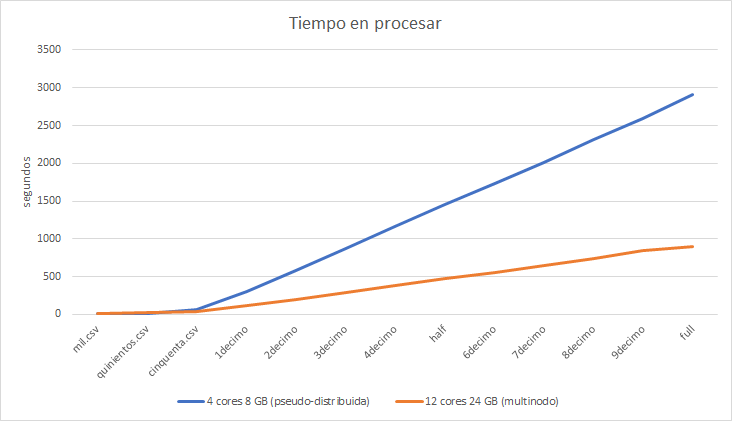
\includegraphics[scale=0.8]{graficas/tpdom}
\end{figure}
\begin{figure}[htp!]
	\centering
	\caption{Gráfica comparativa de la velocidad en el procesamiento de los datos por el clúster doméstico}
	\label{gra:velProcDom}
	\vspace{5pt}
	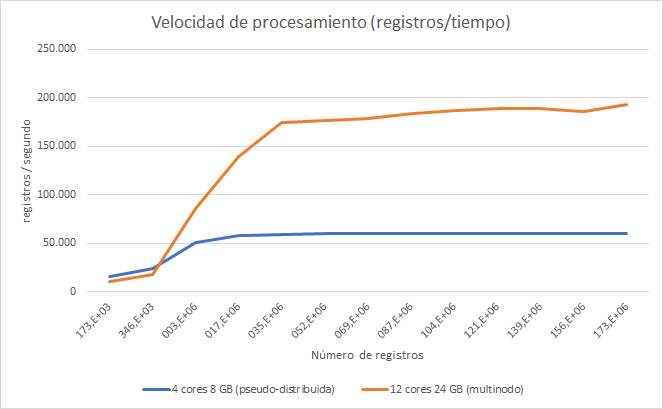
\includegraphics[scale=0.85]{graficas/vpdom}
\end{figure}

En la figura \ref{gra:tiemProcDom} podemos encontrar el tiempo de procesamiento para cada fichero de datos con los que se realizan las pruebas, tanto para el modo pseudo-distribuido (línea azul) como para el modo multinodo (línea naranja). De la misma forma, en la figura \ref{gra:velProcDom} podemos encontrar una gráfica similar pero comparando los registros por segundo que procesa cada configuración.

Ambos resultados resultan acordes con lo esperado, primero, con la propia definición del \textit{big data}, donde estos sistemas no resultan rentables hasta que el volumen de datos es bastante alto. Esto se puede apreciar en ambas gráficas, tanto la de tiempo, como en mayor manera en la de velocidad, donde hasta que no se pasa del millón de registros (a partir del fichero ``cinquenta.csv'') los resultados de ambas configuraciones son muy similares, incluso siendo peor en el caso del multinodo. 

Estos peores resultados en el caso de los ficheros pequeños se puede explicar por el hecho de que el maestro tiene que hacer las distribuciones de los datos entre los tres nodos. Esta transmisión junto con el corto tiempo de ejecución necesario para procesar los mismos hace que la ventaja de añadir capacidad de procesamiento acabe siendo una desventaja al no poder aprovecharse y añadirse al proceso los tiempos de envío de datos.

Sin embargo, es a partir del umbral indicado cuando la velocidad sube en gran manera y se reduce el tiempo de ejecución. Si observamos ambas gráficas, especialmente con el fichero completo, podemos ver que la proporción de tiempo y de registros por segundo es muy similar a la proporción de núcleos de procesamiento de las configuraciones, donde la multinodo tienes tres veces más \gls{CPU}s que la pseudo-distribuida.

Es decir, el tiempo requerido para el procesamiento de la ejecución pseudo-distribuida es casi tres veces mayor que la multinodo. Por otro lado, la cantidad de registros por segundo que procesa la configuración multinodo también es cerca de tres veces mayor. Esto hace pensar que el número de \gls{CPU}s será el factor que influencie los resultados, más que la \gls{RAM}, aunque habrá que confirmarlo con los resultados de las consultas y del clúster universitario.

\begin{figure}[htp!]
	\centering
	\caption{Gráfica comparativa de la eficiencia en el procesamiento de los datos por el clúster doméstico}
	\label{gra:efiProcDom}
	\vspace{5pt}
	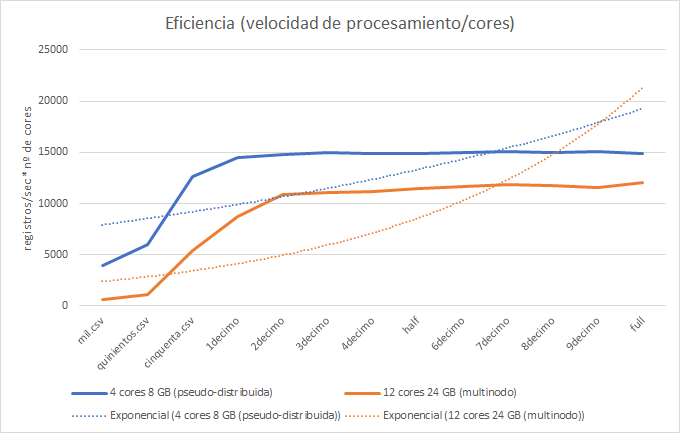
\includegraphics[scale=0.85]{graficas/epdom}
\end{figure}

La figura \ref{gra:efiProcDom} muestra la eficiencia del clúster doméstico en ambas configuraciones. Como se ha explicado anteriormente, la eficiencia es el número de registros que el sistema es capaz de procesar entre el número de \gls{CPU}s de la configuración. En este caso, aparte de apreciar los datos reales, también se ha añadido dos líneas de tendencia para esbozar lo que sucedería si se contase con más datos.

Como apreciamos en la gráfica, vemos como en eficiencia es la configuración pseudo-distribuida la que se muestra por encima en todo momento, queriendo decir que cada núcleo de esta configuración es capaz de procesar más registros por segundo que en el caso de la multinodo. 

Sin embargo, si nos fijamos en la línea de tendencia, vemos como finalmente la configuración multinodo acabaría superando en eficiencia con ficheros con más registros. Este detalle también se puede apreciar con los datos reales, ya que la ejecución pseudo-distribuida se queda estancada a partir del fichero ``2 decimo'' (más de 30 millones de registros) mientras que la multinodo sigue aumentando su eficiencia de forma reducida.

Esto se puede explicar por el proceso de partición de tareas y transmisión de datos, que hace que el sistema tenga que dedicar parte del tiempo de ejecución a establecer las tareas de cada núcleo y a reunir los resultados del procesamiento, haciendo que una configuración donde solo exista un núcleo que tenga que hacer el trabajo sería mejor que otra donde los núcleos se tengan que repartir el trabajo, más si los núcleos están en diferentes computadoras, debido a la latencia de red.

Este efecto solo podría ser contrarrestado, en condiciones normales (donde la partición de tareas y transmisión de datos tomen su tiempo), si la memoria \gls{RAM} dedicada a cada núcleo fuese lo suficientemente grande para albergar todos los datos a procesar y el fichero fuese lo suficientemente grande o si la tarea a realizar necesitase de gran potencia de cálculo.

\subsubsection{Rutas frecuentes}
Para las consultas de rutas frecuentes, como se ha explicado anteriormente (apartado \ref{impConsultas}), existen dos formas de calcularlas. La primera, donde solo se tiene en cuenta la franja de tiempo del día especificado y, otra, donde se da más importancia al día indicado pero también se tienen en cuenta los días iguales cercanos a la fecha introducida, es decir, si se consulta por un viernes, se tienen en cuenta otros viernes cercanos para hacer el cálculo.

\begin{figure}[htp!]
	\centering
	\caption{Gráfica comparativa del tiempo en completar la consulta de rutas frecuentes por el clúster doméstico}
	\label{gra:tiemFreqDom}
	\vspace{5pt}
	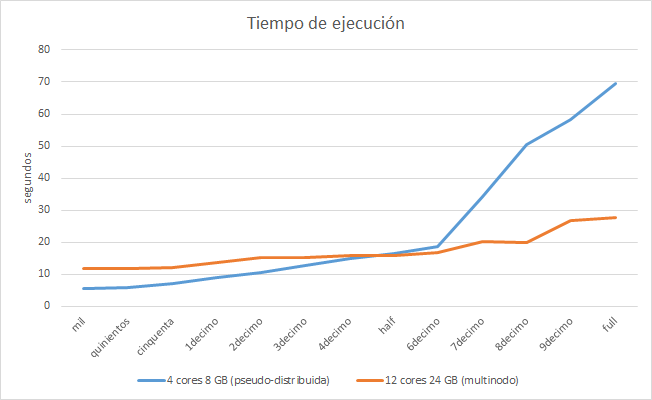
\includegraphics[scale=0.8]{graficas/tfdom}
\end{figure}
\begin{figure}[htp!]
	\centering
	\caption{Gráfica comparativa del tiempo en completar la consulta de rutas frecuentes teniendo en cuenta la estacionalidad por el clúster doméstico}
	\label{gra:tiemFreqDayDom}
	\vspace{5pt}
	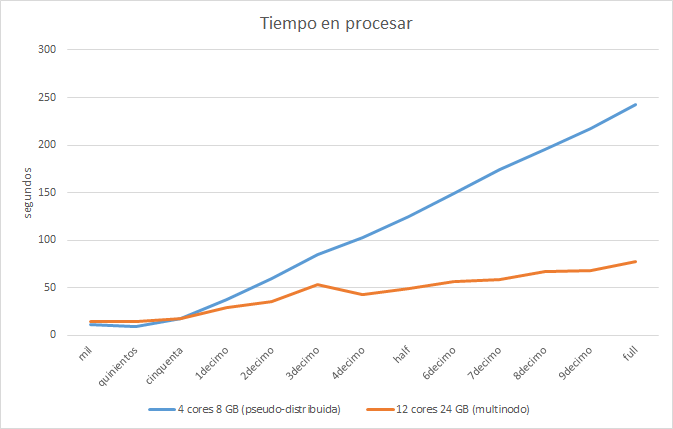
\includegraphics[scale=0.9]{graficas/tfddom}
\end{figure}
\begin{figure}[htp!]
	\centering
	\caption{Gráfica comparativa de la velocidad durante la consulta de rutas frecuentes por el clúster doméstico}
	\label{gra:velFreqDom}
	\vspace{5pt}
	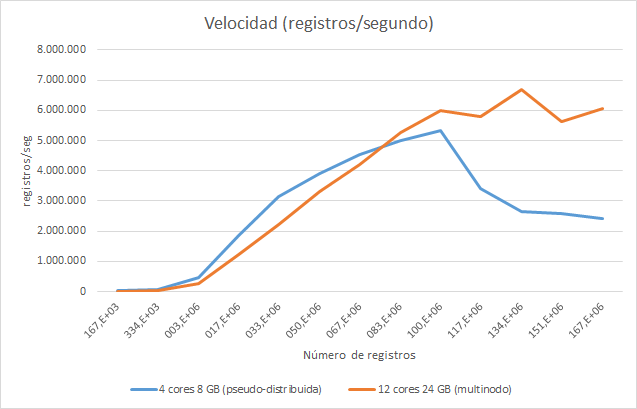
\includegraphics[scale=0.9]{graficas/vfdom}
\end{figure}
\begin{figure}[htp!]
	\centering
	\caption{Gráfica comparativa de la velocidad durante la consulta de rutas frecuentes teniendo en cuenta la estacionalidad por el clúster doméstico}
	\label{gra:velFreqDayDom}
	\vspace{5pt}
	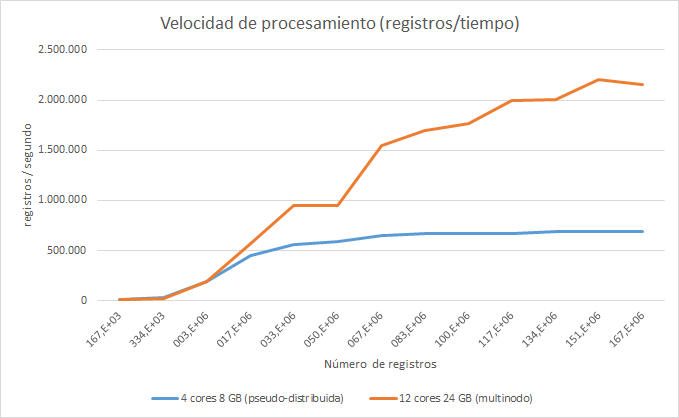
\includegraphics[scale=0.9]{graficas/vfddom}
\end{figure}

La principal diferencia entre estas consultas es el uso de \gls{CPU} necesario, es decir, es la cantidad de cálculos necesarios para obtener los resultados. Aunque ambas realizan un filtrado y una selección, la segunda consulta, al tener en cuenta la estacionalidad, tiene que ponderar las rutas frecuentes de días cercanos, realizando operaciones en como flotante que requieren más cálculos en un ordenador.

Los resultados de tiempo para la primera consulta se pueden apreciar en la figura \ref{gra:tiemFreqDom}, mientras que para la segunda consulta obtenemos los de la figura \ref{gra:tiemFreqDayDom}. Con respecto a la cantidad de registros por segundo de cada consulta, los resultados de la primera se pueden observar en la figura \ref{gra:velFreqDom}, mientras que, los de la segunda están en la figura \ref{gra:velFreqDayDom}.

Si nos paramos a analizar los resultados, la diferencia entre las dos clases es notable, requiriendo bastante menos tiempo la primera consulta, especialmente en el modo pseudo-distribuido. Esto, que arroja una gráfica muy interesante en la figura \ref{gra:tiemFreqDom}, es debido a lo indicado anteriormente sobre los cálculos necesarios para obtener los resultados. En el caso indicado, hasta que no se pasa de los cien millones de registros (fichero ``6decimo'') no es rentable usar una arquitectura \textit{big data} para procesar los datos.

Por otro lado, un aspecto curioso de estas gráficas se encuentra en la figura \ref{gra:velFreqDom} donde la velocidad de la configuración pseudo-distribuida empieza a disminuir a partir de los cien millones de registros en el conjunto de datos, coincidiendo donde empieza a ser rentable el uso de un sistema \textit{big data}. Esta caída del rendimiento es debida a la falta de memoria para almacenar todos los datos en la memoria \gls{RAM} teniendo que acceder al disco para obtener más y, por tanto, produciéndose una ralentización en el proceso. Es aquí donde se puede apreciar de forma clara el efecto de las limitaciones de \gls{RAM}.

Por último, y, en relación a la comparación entre los ficheros \gls{CSV} y los \textit{Parquet} (apartado \ref{compFichDatos}), si comparamos las gráficas de velocidad de estas consultas (figuras \ref{gra:velFreqDom} y \ref{gra:velFreqDayDom}), donde se utiliza \textit{Parquet}, a la de procesamiento de datos (figura \ref{gra:velProcDom}), que lee los \gls{CSV}s originales, se confirma la mayor velocidad de lectura del almacenamiento columnar.

Con respecto a la eficiencia de estas dos consultas, los resultados de la primera se pueden encontrar en la figura \ref{gra:efiFreqDom}, mientras que los de la consulta que tiene en cuenta la estacionalidad se encuentran en la figura \ref{gra:efiFreqDayDom}.

En este caso, para la primera consulta sigue siendo más eficiente el sistema pseudo-distribuido, sin embargo, vemos que para el caso de la segunda consulta esta tendencia cambia a partir del fichero ``8decimo'' que tiene más de 133 millones de registros. Este cambio de tendencia que se produce a partir de este fichero no es debido al tamaño del mismo, si no, como se indicó anteriormente, a la necesidad de cálculo de la consulta para obtener los resultados, que hace que resulte más rentable tener más unidades de procesamiento.

\begin{figure}[htp!]
	\centering
	\caption{Gráfica comparativa de la eficiencia durante la consulta de rutas frecuentes por el clúster doméstico}
	\label{gra:efiFreqDom}
	\vspace{5pt}
	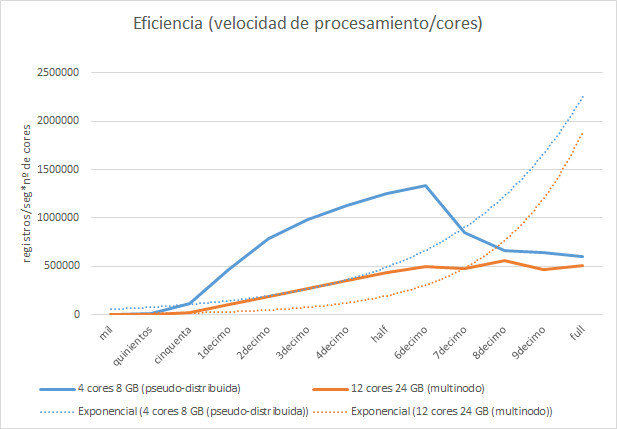
\includegraphics[scale=0.9]{graficas/efdom}
\end{figure}
\begin{figure}[htp!]
	\centering
	\caption{Gráfica comparativa de la eficiencia durante la consulta de rutas frecuentes teniendo en cuenta la estacionalidad por el clúster doméstico}
	\label{gra:efiFreqDayDom}
	\vspace{5pt}
	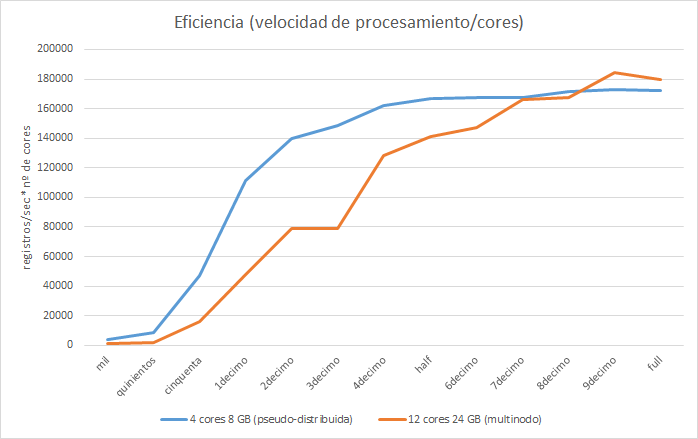
\includegraphics[scale=0.85]{graficas/efddom}
\end{figure}

\subsubsection{Zonas que aportan más beneficios}
Con esta consulta, que calcula las zonas que más beneficios pueden procurarle al taxista a partir de ciertos factores (apartado \ref{profSinExplicacion}), pasa lo mismo que con la consulta de las rutas más frecuentes. Para este trabajo, se han desarrollado dos formas de calcular los datos, la primera teniendo en cuenta solo el día solicitado mientras que, la segunda, tiene en cuenta la estacionalidad.

Estas consultas, que requieren más cálculos que la anterior, acentuará los efectos anteriormente explicados sobre la \gls{CPU}. Además, es este caso, la consulta que tiene en cuenta la estacionalidad es la que más cálculos necesita de las cuatro existentes, representando un ejemplo de uso en un sistema \textit{big data} con gran cantidad de datos e intenso en cálculos.

\begin{figure}[htp!]
	\centering
	\caption{Gráfica comparativa del tiempo en completar la consulta de zonas que reportan más beneficio por el clúster doméstico}
	\label{gra:tiemProDom}
	\vspace{5pt}
	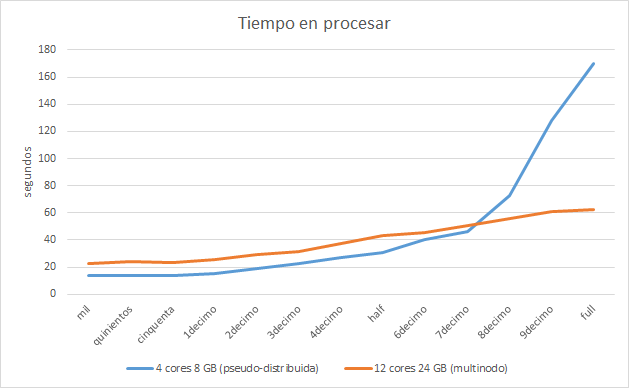
\includegraphics[scale=0.9]{graficas/tbdom}
\end{figure}
\begin{figure}[htp!]
	\centering
	\caption{Gráfica comparativa del tiempo en completar la consulta de zonas que reportan más beneficio teniendo en cuenta la estacionalidad por el clúster doméstico}
	\label{gra:tiemProDayDom}
	\vspace{5pt}
	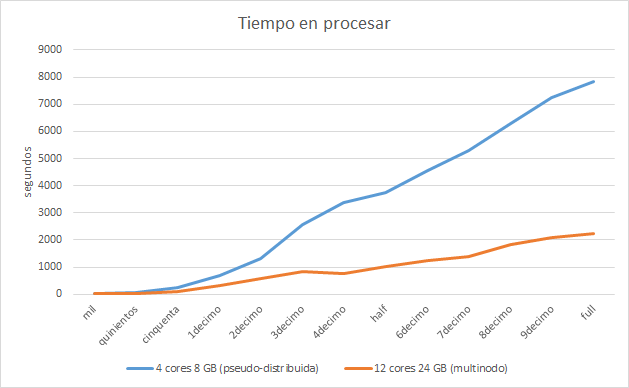
\includegraphics[scale=0.9]{graficas/tbddom}
\end{figure}
\begin{figure}[htp!]
	\centering
	\caption{Gráfica comparativa de la velocidad durante la consulta de zonas que reportan más beneficio por el clúster doméstico}
	\label{gra:velProDom}
	\vspace{5pt}
	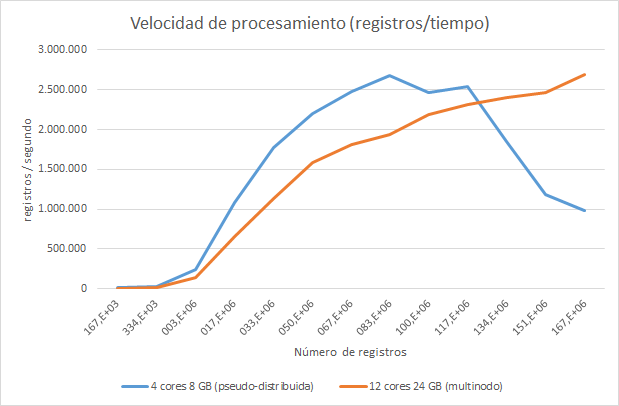
\includegraphics[scale=0.9]{graficas/vbdom}
\end{figure}
\begin{figure}[htp!]
	\centering
	\caption{Gráfica comparativa de la velocidad durante la consulta de zonas que reportan más beneficio teniendo en cuenta la estacionalidad por el clúster doméstico}
	\label{gra:velProDayDom}
	\vspace{5pt}
	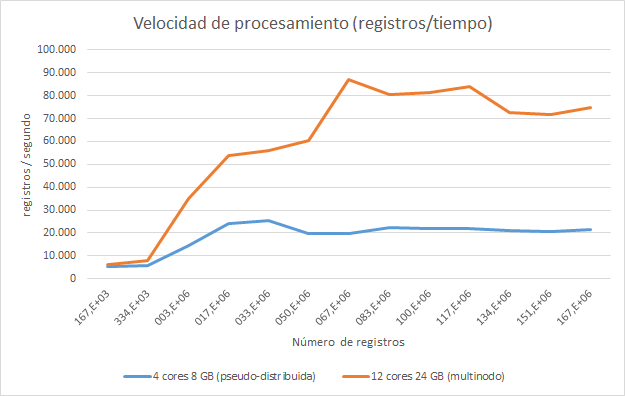
\includegraphics[scale=0.9]{graficas/vbddom}
\end{figure}

En la figuras \ref{gra:tiemProDom} y \ref{gra:velProDom} se pueden observar los resultados de tiempo y velocidad de procesamiento de la primera consulta. Por otro lado, en las figuras \ref{gra:tiemProDayDom} y \ref{gra:velProDayDom} se pueden ver las mismas gráficas para la segunda consulta, que tiene en cuenta la estacionalidad.

Como se ha comentado anteriormente, la segunda consulta es la que más tiempo en realizarse requiere, llegando a necesitar más de dos horas en ejecutarse para la configuración pseudo-distribuida, por el poco más de media hora que requiere hacerlo por la multinodo. Es decir, es en este tipo de tareas tan intensas en cálculo y cantidad de datos donde contar con el extra de \gls{CPU} y memoria \gls{RAM} marcan la diferencia.

Si nos fijamos en la figura \ref{gra:velProDayDom}, donde se representa la velocidad de procesamiento de ambas configuraciones, se puede apreciar que la ejecución multinodo es más veloz desde el comienzo de las pruebas, es decir, con el fichero más pequeño, y, la diferencia entre ambas, comienza a ser notable desde los trescientos mil registros. Esto indica el gran número de operaciones que se realizan para calcular los resultados, al contrario que en los resultados anteriores.

Por otro lado, si nos fijamos en las figuras \ref{gra:tiemFreqDom} y \ref{gra:velFreqDom} que son los resultados de tiempo y velocidad de procesamiento de la consulta que no tiene en cuenta la estacionalidad, al igual que en el caso de las rutas frecuentes, vemos que, a partir del archivo ``6decimo'' que tiene cien millones de registros el tiempo empieza a aumentar de forma brusca y la velocidad se reduce en gran manera.

Esto, al igual que lo explicado anteriormente, pone de manifiesto la importancia de contar con la mayor cantidad de \gls{RAM} posible para evitar los accesos a disco, que bajan el rendimiento en gran manera. En este caso la pérdida de velocidad es de un 60\%, haciendo que el rendimiento del sistema se resienta y los tiempos de ejecución aumenten en una media de dos segundo cada diez millones de registros.

Con respecto a la eficiencia, en la figura \ref{gra:efiFreqDom} se pueden observar los resultados para la primera consulta sobre los beneficios de las zonas y, en la figura \ref{gra:efiFreqDayDom} los de la segunda.

Los resultados obtenidos, en el caso de la primera, se mantienen como en la mayoría de consultas anteriores, donde es más eficiente la configuración pseudo-distribuida para todos los ficheros probados aunque la diferencia al final es reducida y se intuye un cambio de tendencia a mayor número de registros en los datos.

Con respecto a la consulta que tiene en cuenta la estacionalidad, como se intuía en las gráficas anteriores y, debido al alto de número de cálculos que realiza y la gran cantidad de datos a procesar, por primera vez, resulta más rentable la configuración multinodo en la mayoría de los archivos probados.

\begin{figure}[htp!]
	\centering
	\caption{Gráfica comparativa de la eficiencia durante la consulta de zonas que reportan más beneficio por el clúster doméstico}
	\label{gra:efiProDom}
	\vspace{5pt}
	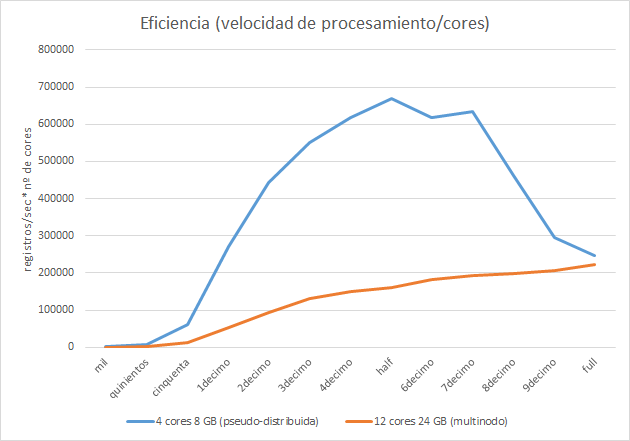
\includegraphics[scale=0.85]{graficas/ebdom}
\end{figure}
\begin{figure}[htp!]
	\centering
	\caption{Gráfica comparativa de la eficiencia durante la consulta de zonas que reportan más beneficio teniendo en cuenta la estacionalidad por el clúster doméstico}
	\label{gra:efiProDayDom}
	\vspace{5pt}
	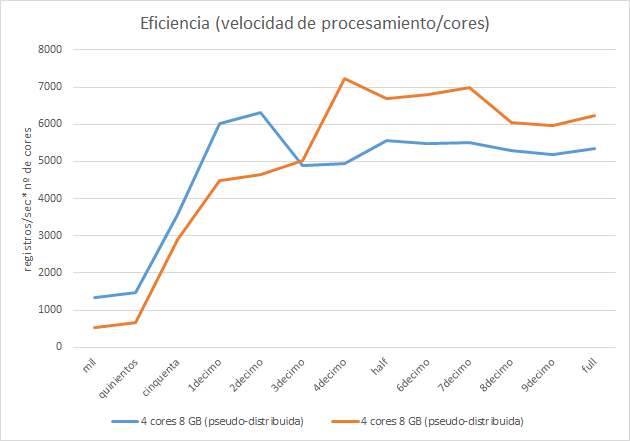
\includegraphics[scale=0.9]{graficas/ebddom}
\end{figure}

\subsection{Clúster universitario}
Tras analizar los resultados del clúster doméstico, en este apartado, se analizarán y estudiaran los resultados obtenidos por el clúster universitario tanto en modo pseudo-distribuido como en el modo multinodo, con las configuraciones indicadas en el apartado \ref{clusterUni}.

Como en el caso anterior, se han realizado las mismas pruebas con los mismos ficheros. La única diferencia es que la prueba de procesamiento de los datos no cuenta con la elaboración de los dos últimos ficheros más grandes, los ficheros ``9decimo'' y ``full'', debido a las limitaciones de cuota de la universidad en los laboratorios.

El punto positivo de este clúster es la homogeneidad de los ordenadores sobre los que se realiza las pruebas, estos, al ser todos iguales, nos permiten realizar pruebas de escalado más precisas, al poder aumentar y reducir las prestaciones del sistema de forma lineal.

En este apartado, las gráficas de eficiencia serán diferentes a las anteriores. Para las realizadas de aquí en adelante se tomaran tres archivos representativos, uno con pocos registros (350.000), otro mediano (51.955.527) y otro más grande (138.548.072), y se comparará la capacidad de procesamiento, en registros por segundo de cada core (velocidad de cada núcleo), para las diferentes configuraciones del multinodo.

Es decir, en el eje $X$ de la gráfica encontraremos el número de cores y, en el eje $Y$, el número de registros por segundo que cada core es capaz de procesar en la configuración. Sin embargo, las gráficas como las del apartado del clúster doméstico estarán situadas en el apéndice \ref{apenEficiencia}. 

\subsubsection{Procesado de datos}
\begin{figure}[htp!]
	\centering
	\caption{Gráfica comparativa del tiempo de procesamiento de los datos por el clúster universitario}
	\label{gra:tiemProcUni}
	\vspace{5pt}
	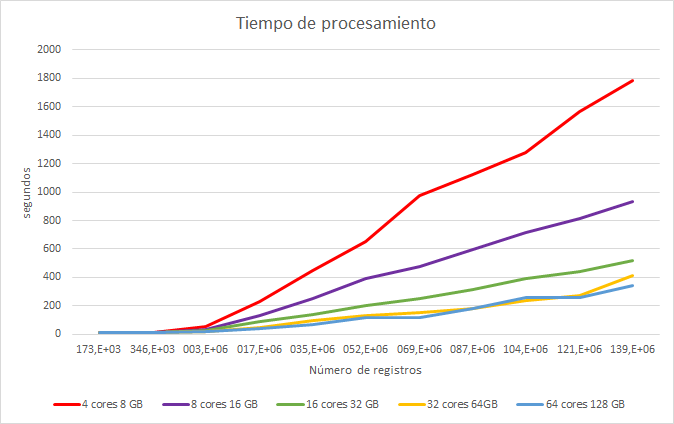
\includegraphics[scale=0.8]{graficas/tpuni}
\end{figure}
\begin{figure}[htp!]
	\centering
	\caption{Gráfica comparativa de la velocidad en el procesamiento de los datos por el clúster universitario}
	\label{gra:velProcUni}
	\vspace{5pt}
	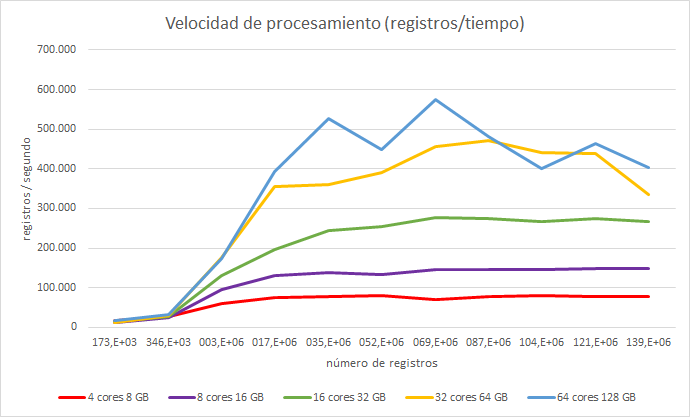
\includegraphics[scale=0.85]{graficas/vpuni}
\end{figure}

Para el procesamiento de datos, como se ha comentado, no se han podido hacer las pruebas con todos los archivos preparados. En este caso, en la figura \ref{gra:tiemProcUni} podemos encontrar los tiempos de ejecución de las diferentes configuraciones utilizadas y, en la figura \ref{gra:velProcUni}, la velocidad de procesamiento.

Primero, si nos fijamos en los tiempos de procesamiento de las diferentes configuraciones podemos apreciar con claridad el efecto, comentado anteriormente, que produce la transmisión de los datos entre los dispositivos del clúster. Es decir, el cuello de botella que produce la transmisión de las tareas por la red, que hace que los tiempos no se reduzcan proporcionalmente a la potencia.

En este caso, para más de 130 millones de registros, podemos observar que al pasar de la configuración pseudo-distribuida, 4 cores y 8 \gls{GB}, a la primera multinodo, 8 cores y 16 \gls{GB}, el tiempo de la tarea se reduce prácticamente a la mitad, de los 1800 segundos a poco más de 900. En el paso de esta primera configuración a la segunda, 16 cores y 32 GB, también reduce prácticamente a la mitad del tiempo, de 900 segundos a cerca de 500.

Sin embargo, a partir de este momento, la capacidad de procesamiento añadida por el resto de configuraciones no compensa al efecto producido por la comunicación entre los nodos. Especial ejemplo de esto es la diferencia casi nula entre los tiempos de la configuración con 8 y 16 nodos.

Este efecto también se puede apreciar en la figura \ref{gra:velProcUni}, que muestra la velocidad de procesamiento, donde, aunque la capacidad aumenta con cada configuración con más nodo, esta en ningún caso llega al teórico caso de doblar su potencia. 

\begin{figure}[htp!]
	\centering
	\caption{Gráfica comparativa de la eficiencia en el procesamiento de los datos por el clúster universitario}
	\label{gra:efiProcUni}
	\vspace{5pt}
	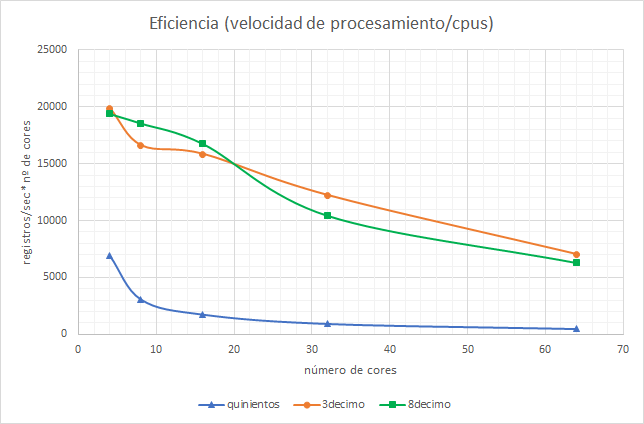
\includegraphics[scale=0.85]{graficas/epuni2}
\end{figure}

Con respecto a la eficiencia de las diferentes configuraciones, podemos apreciar los resultados en la figura \ref{gra:efiProcUni}, donde se puede comparar la velocidad de cada core para las diferentes configuraciones multinodo. En ella podemos apreciar, de nuevo, que añadir más cores al sistema no implica una mayor capacidad de procesamiento debido al coste de la transmisión de datos.

\subsubsection{Rutas más frecuentes}
\begin{figure}[htp!]
	\centering
	\caption{Gráfica comparativa del tiempo en completar la consulta de rutas frecuentes por el clúster universitario}
	\label{gra:tiemFreqUni}
	\vspace{5pt}
	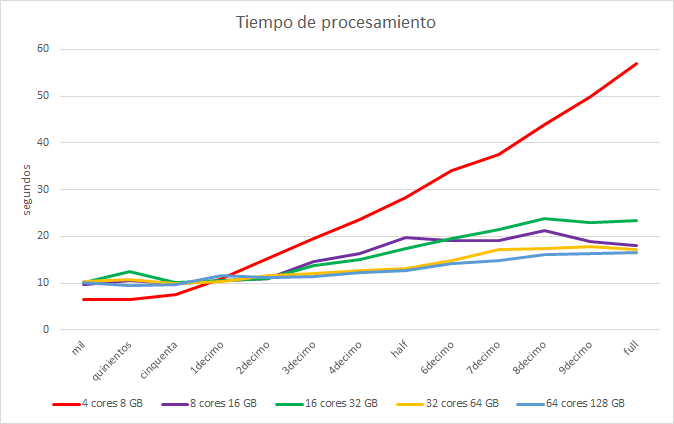
\includegraphics[scale=0.85]{graficas/tfuni}
\end{figure}
\begin{figure}[htp!]
	\centering
	\caption{Gráfica comparativa del tiempo en completar la consulta de rutas frecuentes teniendo en cuenta la estacionalidad por el clúster universitario}
	\label{gra:tiemFreqDayUni}
	\vspace{5pt}
	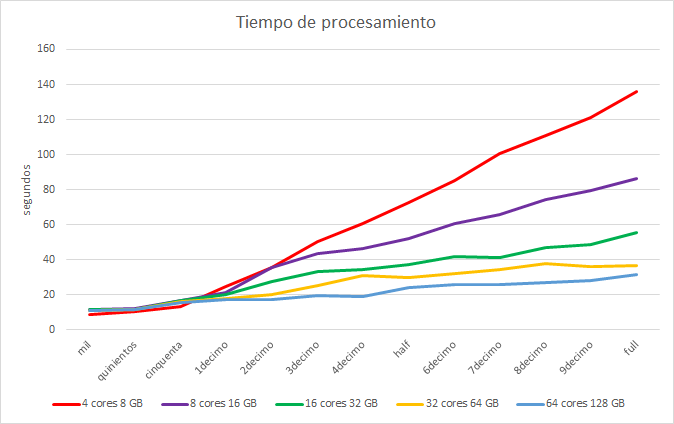
\includegraphics[scale=0.85]{graficas/tfduni}
\end{figure}
\begin{figure}[htp!]
	\centering
	\caption{Gráfica comparativa de la velocidad durante la consulta de rutas frecuentes por el clúster universitario}
	\label{gra:velFreqUni}
	\vspace{5pt}
	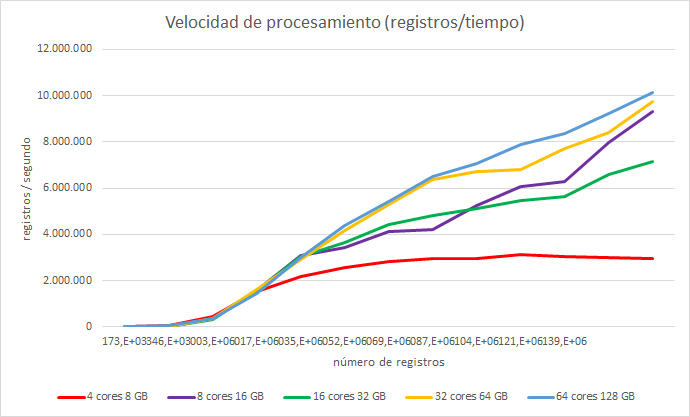
\includegraphics[scale=0.8]{graficas/vfuni}
\end{figure}
\begin{figure}[htp!]
	\centering
	\caption{Gráfica comparativa de la velocidad durante la consulta de rutas frecuentes teniendo en cuenta la estacionalidad por el clúster universitario}
	\label{gra:velFreqDayUni}
	\vspace{5pt}
	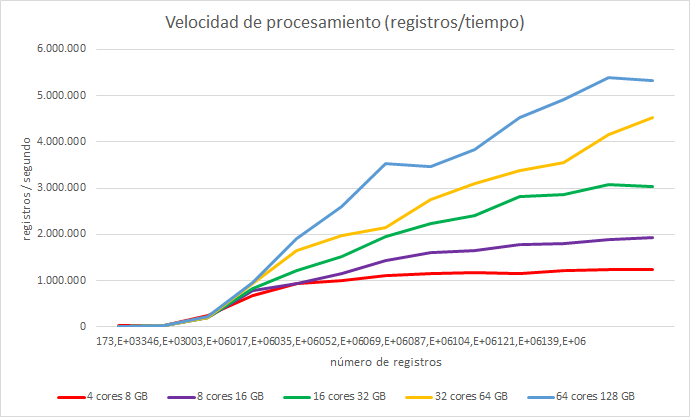
\includegraphics[scale=0.9]{graficas/vfduni}
\end{figure}

Para el clúster universitario, igual que para el doméstico, también se ejecutarán las dos consultas que devuelven la información de las rutas frecuentes. La gráfica con los resultados de tiempos se pueden observar en la figura \ref{gra:tiemFreqUni} para la primera consulta y en la figura \ref{gra:tiemFreqDayUni} para la segunda. Con respecto a la de velocidad de procesamiento, la figura \ref{gra:velFreqUni} para la primera consulta y, para la que tiene en cuenta la estacionalidad, en la figura \ref{gra:velFreqDayUni}.

Si comenzamos analizando la gráfica de tiempos de la primera consulta, figura \ref{gra:tiemFreqUni}, se ve con mayor claridad lo ya explicado anteriormente sobre esta consulta. Al tratarse de un simple filtrado de registros dentro de un franja horaria, para archivos de datos pequeños la configuración pseudo-distribuida es más rápida que cualquiera multinodo, debido al coste de la distribución de las tareas y datos por la red. Sin embargo, vemos como que para archivos mayores esta tendencia cambia y las configuraciones multinodo son el doble de rápidas. Para el archivo ``full'', cerca de 60 segundos para la configuración pseudo-distribuida por los poco más de 20 segundos de la peor multinodo.

La naturaleza de la consulta y el coste de la comunicación entre los nodos es también la culpable de que todas las configuraciones multinodo estén en un rango de 10 segundos [23,34 seg - 16,54 seg] no resultando efectivo añadir más cores al sistema. Esta similitud de procesamiento también se puede apreciar en la figura \ref{gra:velFreqUni}, que muestra como la configuración con dos nodos es superior a la de cuatro en velocidad de procesamiento.

Con respecto a la segunda consulta, cuyos datos se pueden encontrar en las figuras \ref{gra:tiemFreqDayUni} y \ref{gra:velFreqDayUni}, apreciamos que se cumple lo explicado en los resultados del clúster doméstico. Debido a la mayor cantidad de cálculos necesarios por esta, los tiempos de procesamiento son mayores que en la otra consulta y, por ello, la diferencia entre las configuraciones es más notable, produciéndose mejorías cercanas al 50\% hasta las dos últimas, con 8 y 16 nodos, donde la diferencia es de 5 segundos.

\begin{figure}[htp!]
	\centering
	\caption{Gráfica comparativa de la eficiencia durante la consulta de rutas frecuentes por el clúster universitario}
	\label{gra:efiFreqUni}
	\vspace{5pt}
	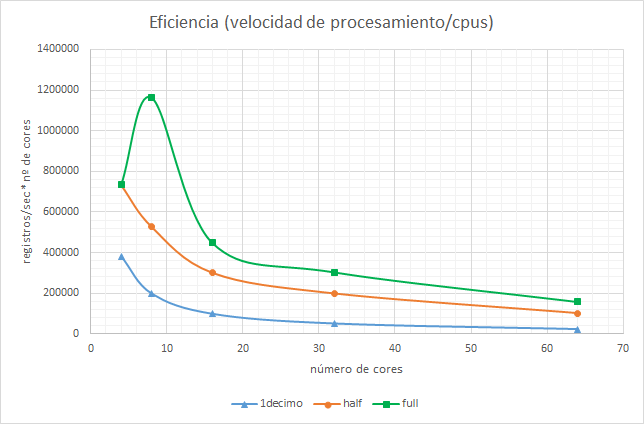
\includegraphics[scale=0.9]{graficas/efuni2}
\end{figure}
\begin{figure}[htp!]
	\centering
	\caption{Gráfica comparativa de la eficiencia durante la consulta de rutas frecuentes teniendo en cuenta la estacionalidad por el clúster universitario}
	\label{gra:efiFreqDayUni}
	\vspace{5pt}
	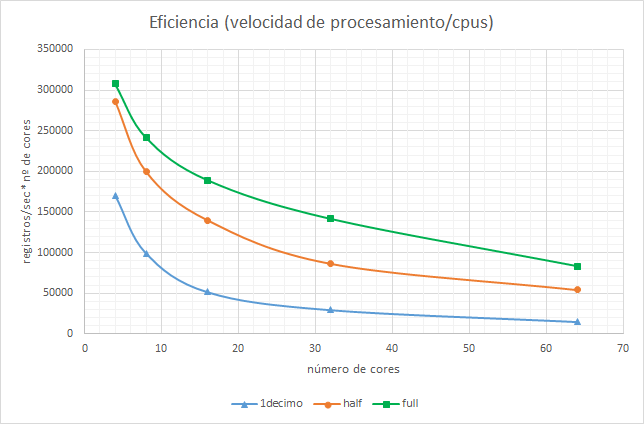
\includegraphics[scale=0.9]{graficas/efduni2}
\end{figure}

En cuanto a la eficiencia, en la figura \ref{gra:efiFreqUni} se pueden observar los datos con respecto al número de cores de las configuraciones probadas de la primera consulta. En este caso, lo más interesante de la gráfica se produce para la configuración de dos nodos (ocho cores) para el archivo completo, donde se produce una subida de la eficiencia, en discordancia con lo visto hasta ahora.

Este detalle concuerda con los resultados obtenidos en las figura \ref{gra:tiemFreqUni} y \ref{gra:velFreqUni}, donde se observa que la configuración de 2 nodos es superior a la de 4 en ficheros grandes. Esto puede deberse a que la partición de datos entre los nodos aprovecha de forma optima la memoria \gls{RAM} del sistema y obtiene buenos resultados debido a la minimización que se produce sobre el coste de la comunicación en red.

Con respecto a la segunda consulta, los resultados obtenidos se pueden encontrar en la figura \ref{gra:efiFreqDayUni}, que mantiene lo explicado anteriormente.

\subsubsection{Zonas que aportan más beneficios}
\begin{figure}[htp!]
	\centering
	\caption{Gráfica comparativa del tiempo en completar la consulta de zonas que reportan más beneficio por el clúster universitario}
	\label{gra:tiemProUni}
	\vspace{5pt}
	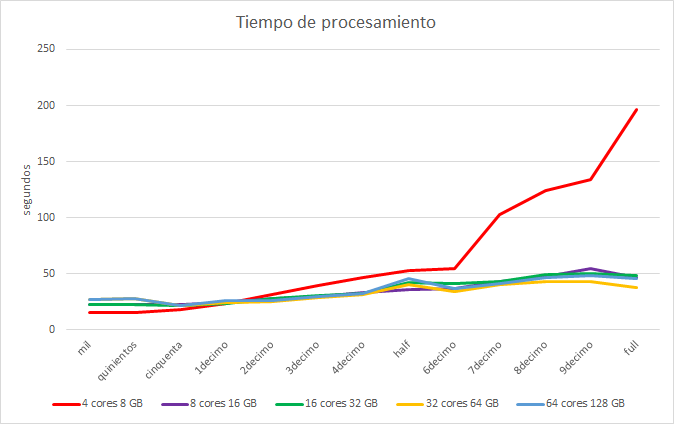
\includegraphics[scale=0.85]{graficas/tbuni}
\end{figure}
\begin{figure}[htp!]
	\centering
	\caption{Gráfica comparativa del tiempo en completar la consulta de zonas que reportan más beneficio teniendo en cuenta la estacionalidad por el clúster universitario}
	\label{gra:tiemProDayUni}
	\vspace{5pt}
	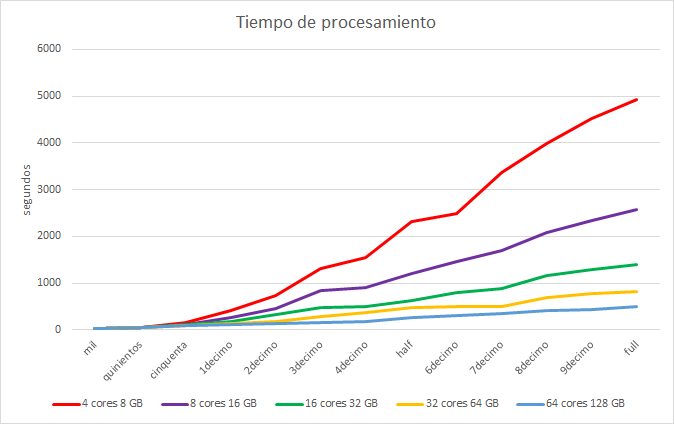
\includegraphics[scale=0.85]{graficas/tbduni}
\end{figure}
\begin{figure}[htp!]
	\centering
	\caption{Gráfica comparativa de la velocidad durante la consulta de zonas que reportan más beneficio por el clúster universitario}
	\label{gra:velProUni}
	\vspace{5pt}
	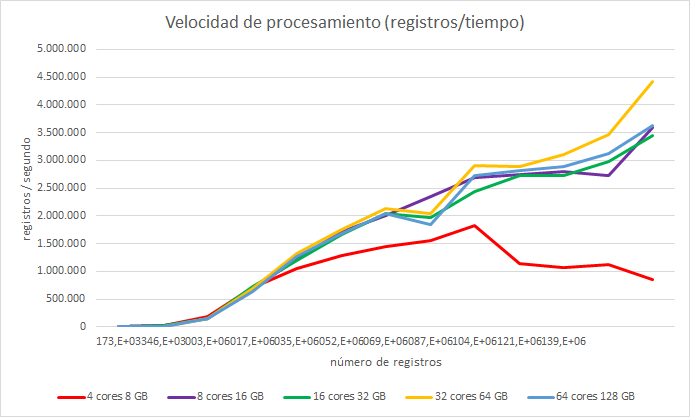
\includegraphics[scale=0.85]{graficas/vbuni}
\end{figure}
\begin{figure}[htp!]
	\centering
	\caption{Gráfica comparativa de la velocidad durante la consulta de zonas que reportan más beneficio teniendo en cuenta la estacionalidad por el clúster universitario}
	\label{gra:velProDayUni}
	\vspace{5pt}
	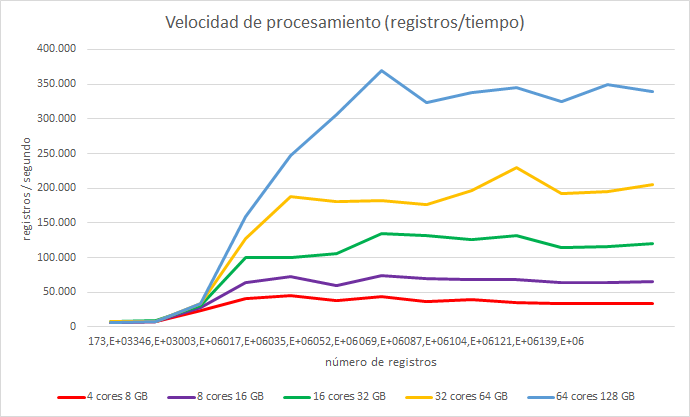
\includegraphics[scale=0.85]{graficas/vbduni}
\end{figure}

En este caso, como con el clúster doméstico, se han ejecutado las dos consultas para obtener las zonas que más beneficio pueden aportar al taxista. Los tiempos de ejecución de la primera, que solo tiene en cuenta la franja horaria deseada, obtiene los tiempos de ejecución que se pueden observar en la figura \ref{gra:tiemProUni}.

Si analizamos estos resultados, vemos que son muy similares a los obtenidos por el clúster doméstico (figura \ref{gra:tiemFreqDom}) donde la diferencia de tiempos entre el modo pseudo-distribuido y el multinodo es casi nula hasta el fichero ``6decimo'' y, tras este, la diferencia se vuelve muy abrupta. Esto también se puede apreciar en la tabla de resultados de la velocidad de procesamiento, figura \ref{gra:velProUni}.

Como se explicó en aquel caso, esto es debido a la falta de memoria \gls{RAM} para almacenar los datos completos, haciendo que sea necesario el acceso a disco y, por tanto, reduciendo la capacidad del sistema. Con respecto a las diferentes configuraciones multinodo, estas mantienen resultados de tiempo y velocidad de procesamiento muy similares, indicando que el uso de \gls{CPU} para cálculo no es suficiente para contrarrestar el coste de la comunicación entre los nodos.

Esto último cambia en el caso de la segunda consulta, donde si se tiene en cuenta la estacionalidad y, por tanto, el número de cálculos necesarios para obtener los resultados es mucho mayor, como se vio en el clúster doméstico. En este caso, los resultados se puede encontrar en la figura \ref{gra:tiemProDayUni} en el caso del tiempo de ejecución y, en la figura \ref{gra:velProDayUni}, para la velocidad de procesamiento.

En este caso, como en el caso del clúster doméstico, es donde se saca el mayor rendimiento a la arquitectura \textit{big data}. Si observamos la tabla \ref{t:tiemfull}, que contiene los tiempos de cada configuración del clúster junto con la diferencia de tiempo con respecto a la configuración anterior en potencia, podemos observar como los tiempos se reducen en más de un 50\% con respecto a su predecesor en potencia.

\begin{table}[htp!]
	\centering
	\caption{Tiempos clúster universitario para archivo ``full'' y diferencia con respecto a la anterior configuración menos potente}
	\label{t:tiemfull}
	\begin{tabular}{|c|c|c|}
		\hline
		\multicolumn{1}{|l|}{}   & \textbf{Tiempo} & \textbf{Diferencia} \\ \hline
		\textbf{4 cores 8 GB}    & 4924,275306     & 100                 \\ \hline
		\textbf{8 cores 16 GB}   & 2566,806429     & 52,1255671          \\ \hline
		\textbf{16 cores 32 GB}  & 1398,539243     & 54,48557504         \\ \hline
		\textbf{32 cores 64 GB}  & 814,9681364     & 58,27281147         \\ \hline
		\textbf{64 cores 128 GB} & 493,53187       & 60,55842529         \\ \hline
	\end{tabular}
\end{table}

Esto resultados representan el funcionamiento ideal de la arquitectura \textit{big data} y se producen debido al alto requerimiento en potencia de cálculo de esta consulta, que realiza varios \textit{joins} de tablas entre los cálculos parciales que efectúa, siendo esta operación muy costosa y consiguiendo contrarrestar, en parte, el coste de la comunicación y envío de los datos por la red.

\begin{figure}[htp!]
	\centering
	\caption{Gráfica comparativa de la eficiencia durante la consulta de zonas que reportan más beneficio por el clúster universitario}
	\label{gra:efiProUni}
	\vspace{5pt}
	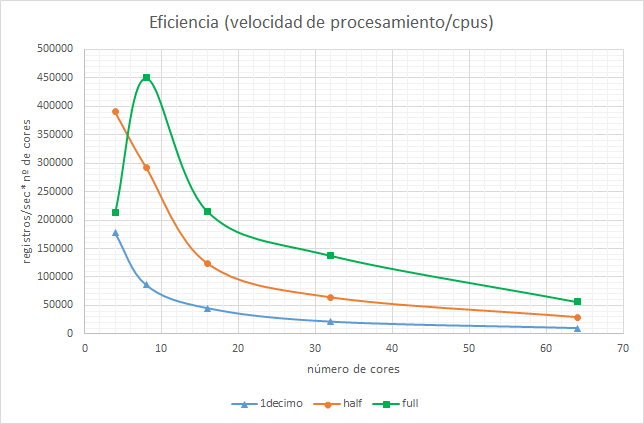
\includegraphics[scale=0.85]{graficas/ebuni2}
\end{figure}
\begin{figure}[htp!]
	\centering
	\caption{Gráfica comparativa de la eficiencia durante la consulta de zonas que reportan más beneficio teniendo en cuenta la estacionalidad por el clúster universitario}
	\label{gra:efiProDayUni}
	\vspace{5pt}
	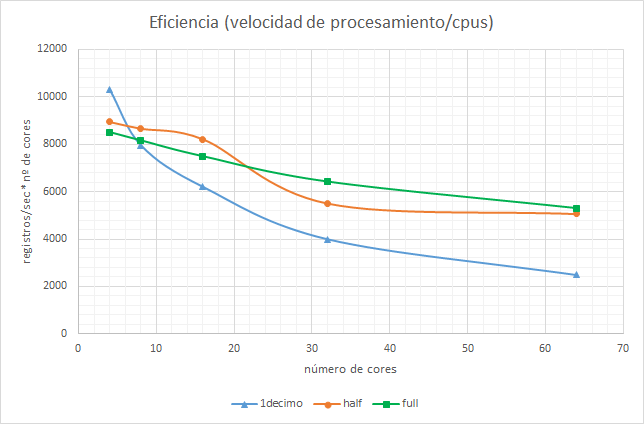
\includegraphics[scale=0.9]{graficas/ebduni2}
\end{figure}

Con respecto a la eficiencia, en el caso de la primera consulta, cuyos resultados se pueden observar en la figura \ref{gra:efiProUni}, son muy similares a lo visto anteriormente, teniendo gran similitud con los resultados obtenidos en la primera consulta de las rutas más frecuentes (figura \ref{gra:efiFreqUni}).

En cuanto a la segunda consulta, cuyos resultados se encuentran en la figura \ref{gra:efiFreqDayUni}, podemos observar como realmente el coste de la transmisión de los datos no es contrarrestado totalmente por la cantidad de cálculos de la consulta, ya que, es más eficiente la configuración pseudo-distribuida en cuanto al procesamiento de registros por segundo en cada core.

Sin embargo, comparado con los resultados obtenidos hasta ahora en cuanto a eficiencia, sí se puede observar el menor grado de la pendiente entre configuraciones con más cores, es decir, la potencia perdida es menor en este caso, debido a la alta cantidad de cálculos que hay que llevar a cabo.

\subsection{Conclusiones sobre el rendimiento}
Tras haber realizado las pruebas en ambos clústeres y analizar los resultados, podemos extraer varias conclusiones. La primera es que hay que tener en cuenta la latencia de red para el diseño del sistema \textit{big data}, ya que, no siempre tener mayor potencia bruta (más núcleos y memoria RAM) implica una mejor respuesta en cuanto a capacidad de procesamiento.

Es decir, hemos visto como, dependiendo de la naturaleza, era hasta negativo añadir más nodos al sistema. Por ello, hay que buscar un equilibrio entre la latencia introducida por la transmisión de los datos en la red y la capacidad de procesamiento añadida de los nodos.

Por otro lado, debido a las decisiones de diseño tomadas en la creación de este sistema \textit{big data}, hemos observado como el número de núcleos resultaba siendo más determinante que la cantidad de memoria \gls{RAM}. Esto se ha debido al mecanismo de compresión utilizado, que, por un lado, requería capacidad de procesamiento para las tareas de descompresión de los ficheros de datos y, por otro, reducía el tamaño de los ficheros de datos, que se podían mantener comprimidos en la memoria \gls{RAM} de los equipos al ser de menor tamaño que sus capacidad total.

Sin embargo, hemos visto como la \gls{RAM} hubiese sido determinante si el tamaño de los datos hubiera sido mayor, ya que en casos como los analizados en la figura \ref{gra:tiemProUni}, en cuanto el sistema se quedaba sin espacio para almacenar los datos y los resultados intermedios en la \gls{RAM}, el rendimiento del sistema se veía fuertemente castigado por los accesos a disco, que son mucho más lentos.

Por tanto, tras expuesto anteriormente, en el proceso de diseño e implementación de un sistema \textit{big data} una de las tareas más importantes es analizar la naturaleza de la tarea que se realizará para poder establecer un equilibrio eficiente entre la capacidad de cómputo de los nodos y la latencia de red. Además, se debe procurar aprovechar al máximo la memoria \gls{RAM} y evitar los accesos a discos, ya sea introduciendo grandes cantidades de \gls{RAM} al sistema o mediante mecanismos de compresión, si la capacidad de cómputo del sistema es suficiente.
